\documentclass[10pt,aspectratio=43]{beamer}

\usepackage{graphicx}
\usepackage{tikz}
\usepackage{xcolor}
\usepackage{caption}
\usepackage{subcaption}
\usepackage{bm}
\usetikzlibrary{calc} 
\usepackage{hyperref}
\hypersetup{
    colorlinks=true,
    linkcolor=blue,
    urlcolor=red
}
\usepackage{fontawesome5}
\usepackage{ulem}
\usepackage[dvipsnames]{xcolor}

\usetheme{MyStyle}   % loads beamerthemeMyStyle.sty
\setlength{\columnsep}{0pt}


%%%%%%%%%%%%%%%%%%%%%%%%%%%%%%%%%%%%%%%%%%
%%%%%%%%%%%%%%%%%%%%%%%%%%%%%%%%%%%%%%%%%%
%%%%%%%%%%%%%%%%%%%%%%%%%%%%%%%%%%%%%%%%%%

\title{Efficiency of the time reconstruction \\ of saturated signals}
\newcommand{\eventname}{ALERT meeting}
\author{Felix Touchte Codjo}
\institute{IJCLab}
\date{\today}


\begin{document}

\begin{frame}[plain] % remove header, footer, barre de navigation
\titlepage
\end{frame}

%\begin{frame}{Outline}
%\tableofcontents
%\end{frame}

%\section{Intro}
\section{Updates}



\begin{frame}{Reminder}
    \begin{itemize}
        \item The amplitude of saturated signals can be estimated using
    \end{itemize}

    \begin{equation*}
        \bm{ADC}_{corr} = f (\bm{slope}) 
    \end{equation*}

    where $f$ is extracted from non-saturated signals

    \centering
    \vspace{0.5cm}

    % \begin{figure}
    %     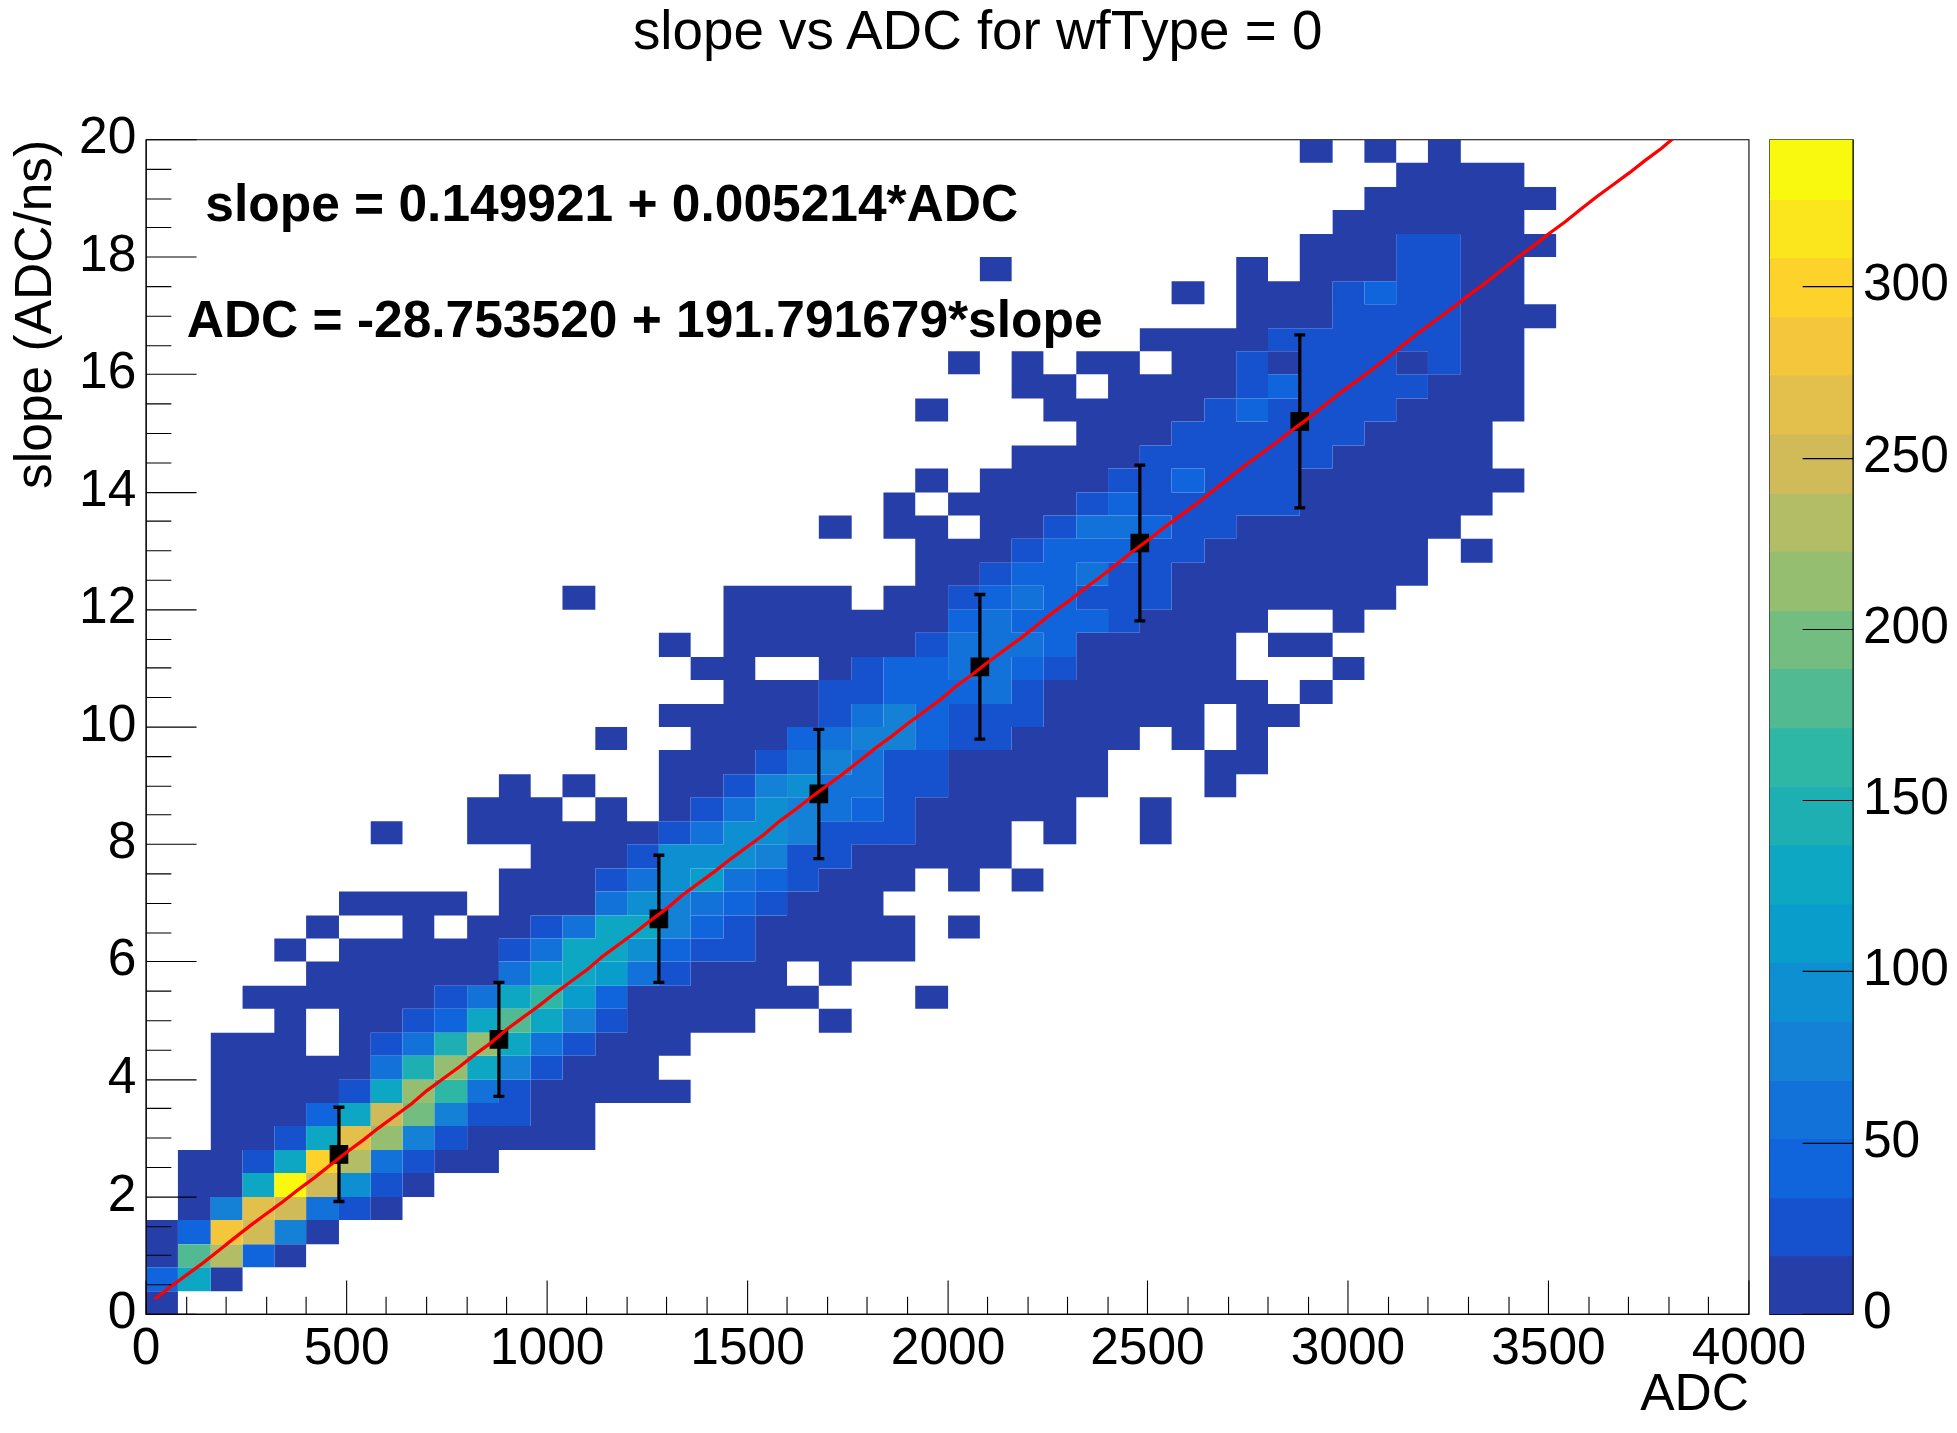
\includegraphics[width=0.5\linewidth]{figures/fit_adc_versus_slope.png}
    % \end{figure}

    \begin{tabular}{cc}
        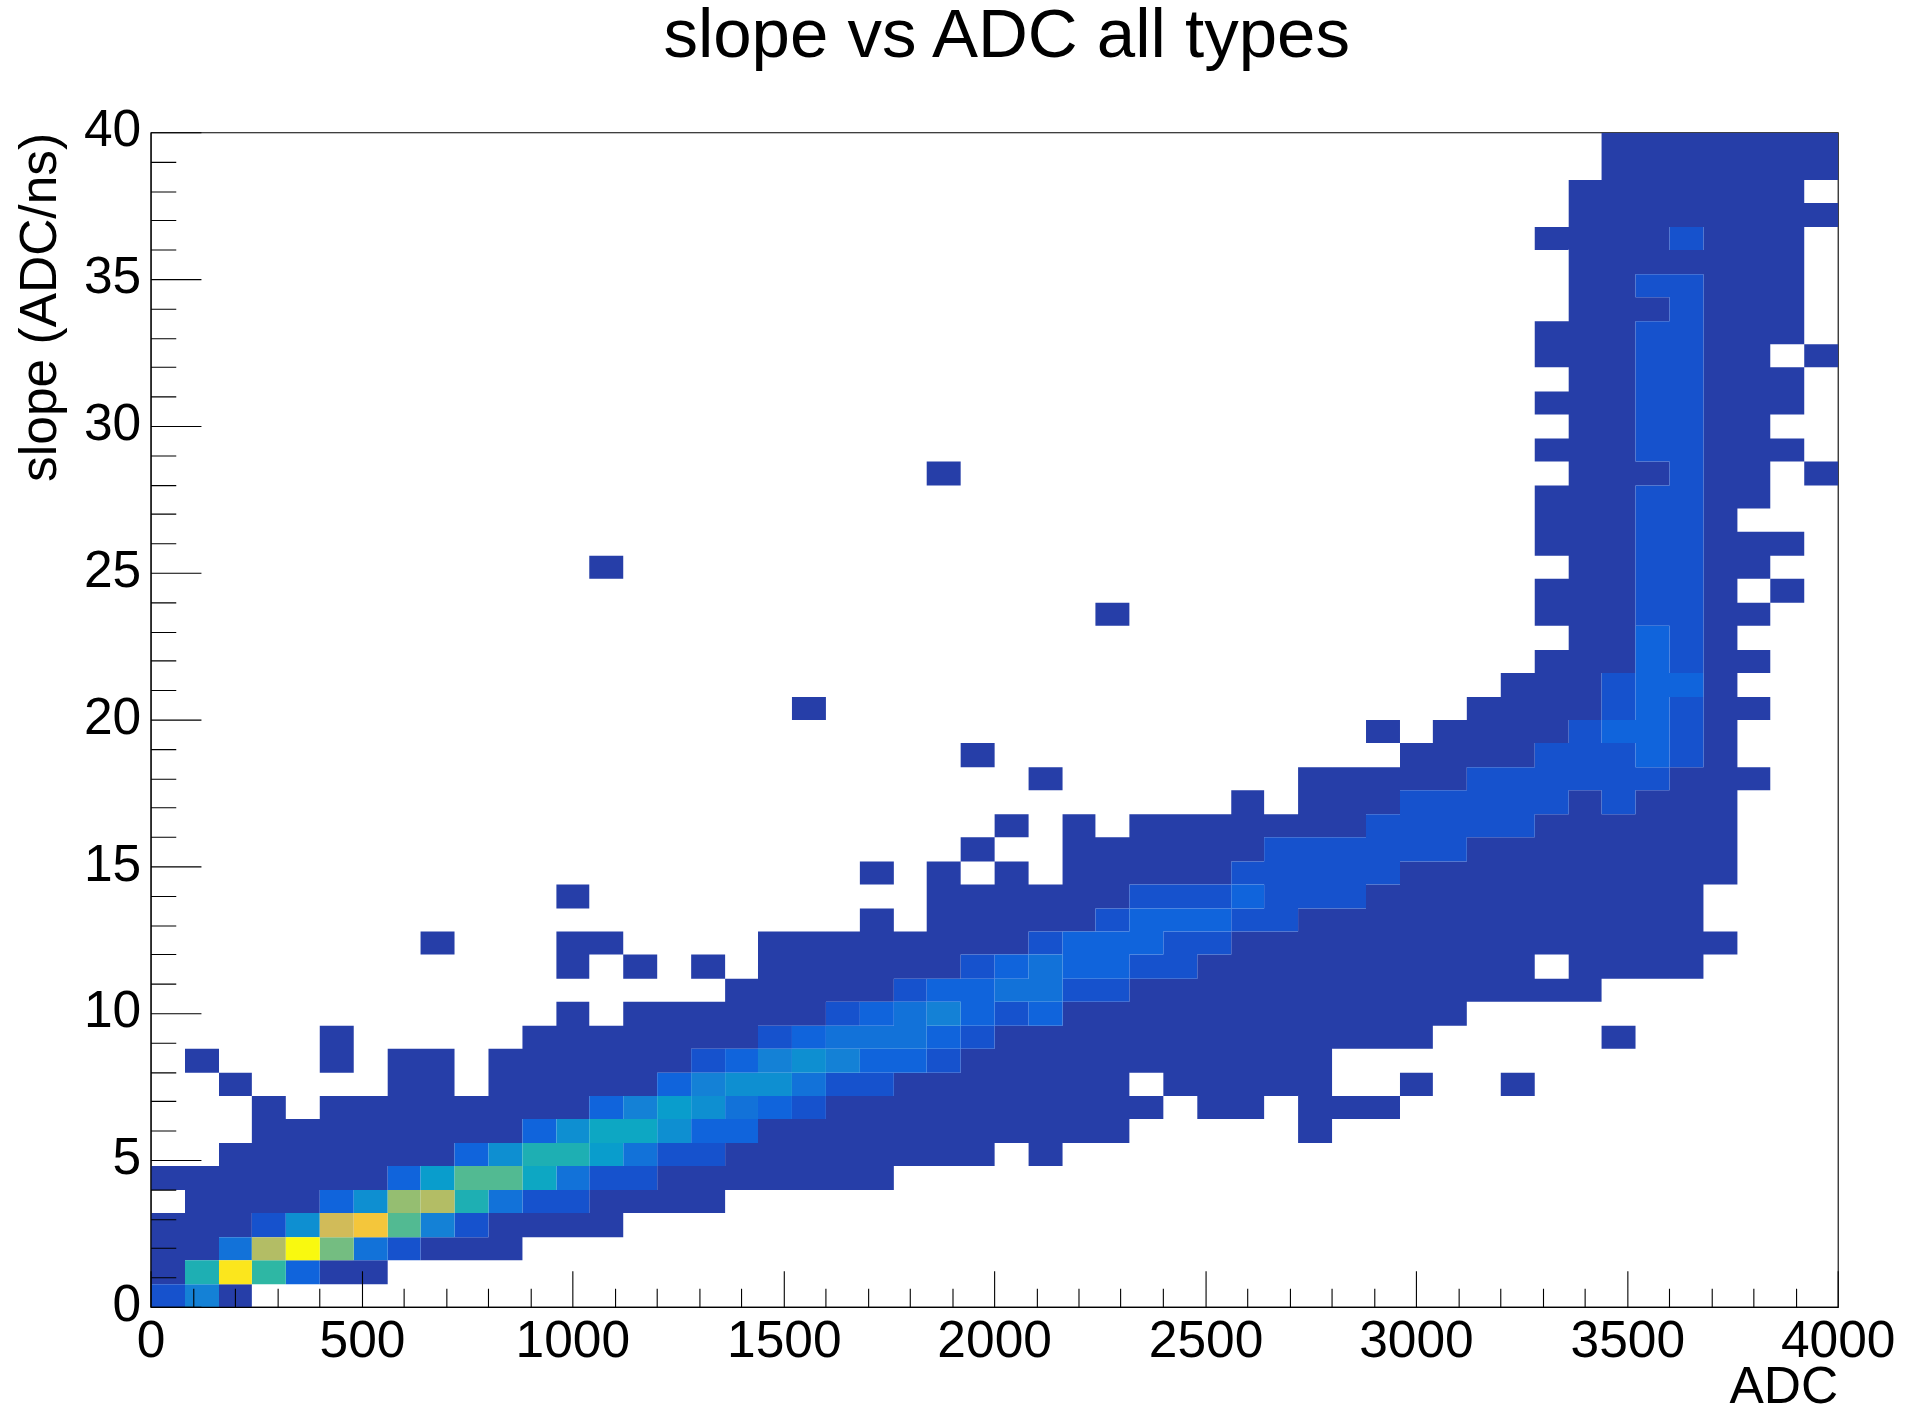
\includegraphics[width=0.45\linewidth]{figures/slope_vs_adc_all_wf.png} &
            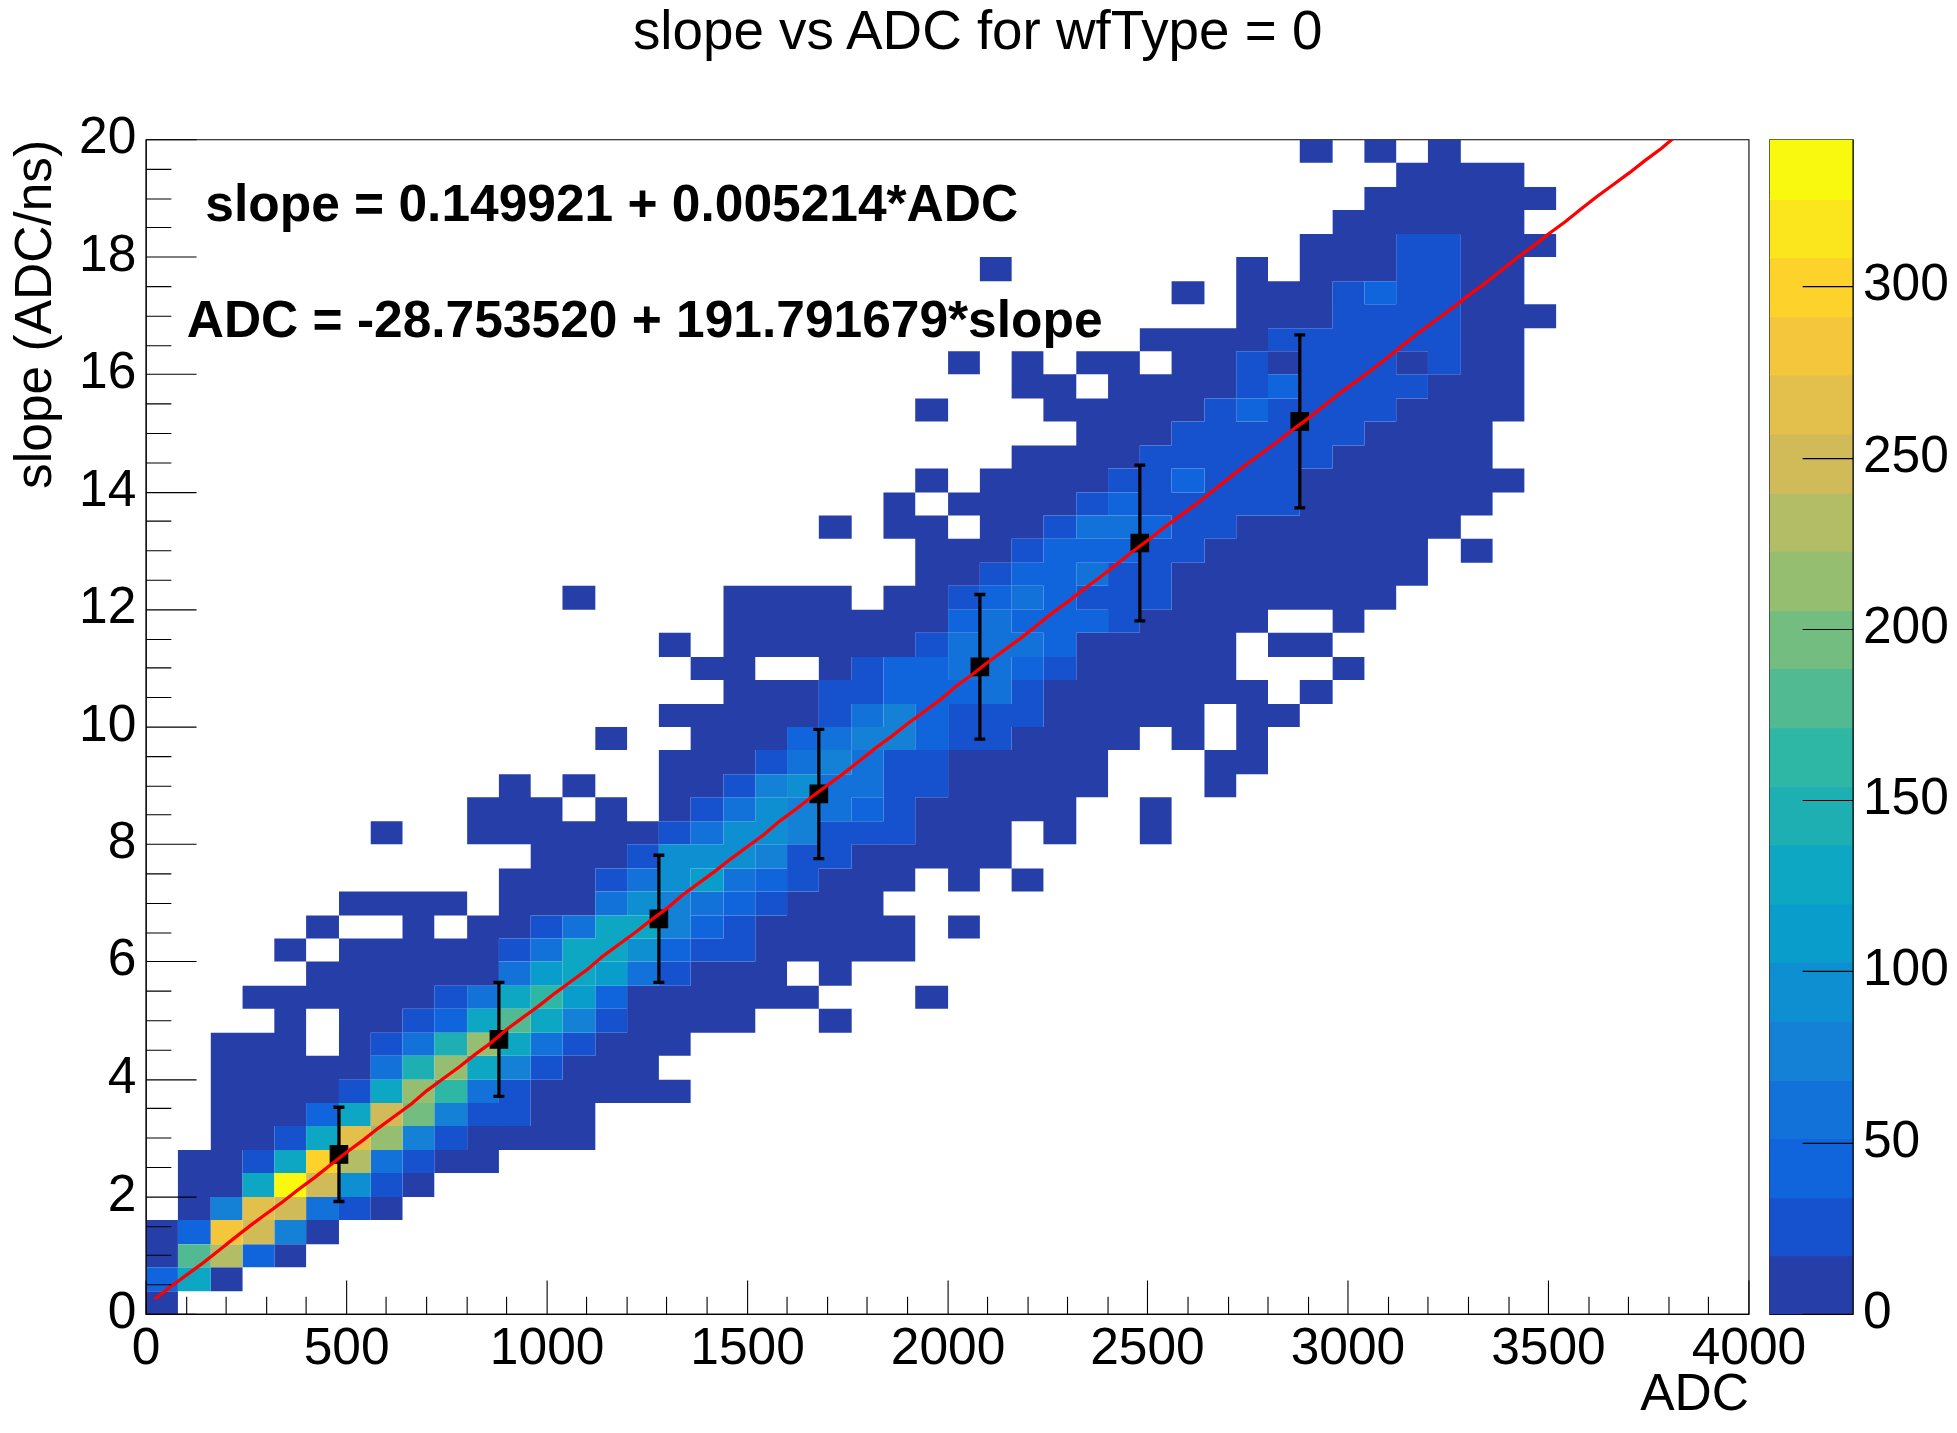
\includegraphics[width=0.45\linewidth]{figures/fit_adc_versus_slope.png}
    \end{tabular}

\end{frame}

\begin{frame}{Results 1/2}
    \begin{itemize}
        \item Once we have a reasonable estimate of the amplitude, we can re-compute the time at half amplitude
        \item We no longer have the accumulation of small time at 3500 ADC
    \end{itemize}

    \centering
    \vspace{0.2cm}

    \begin{tabular}{cc}
        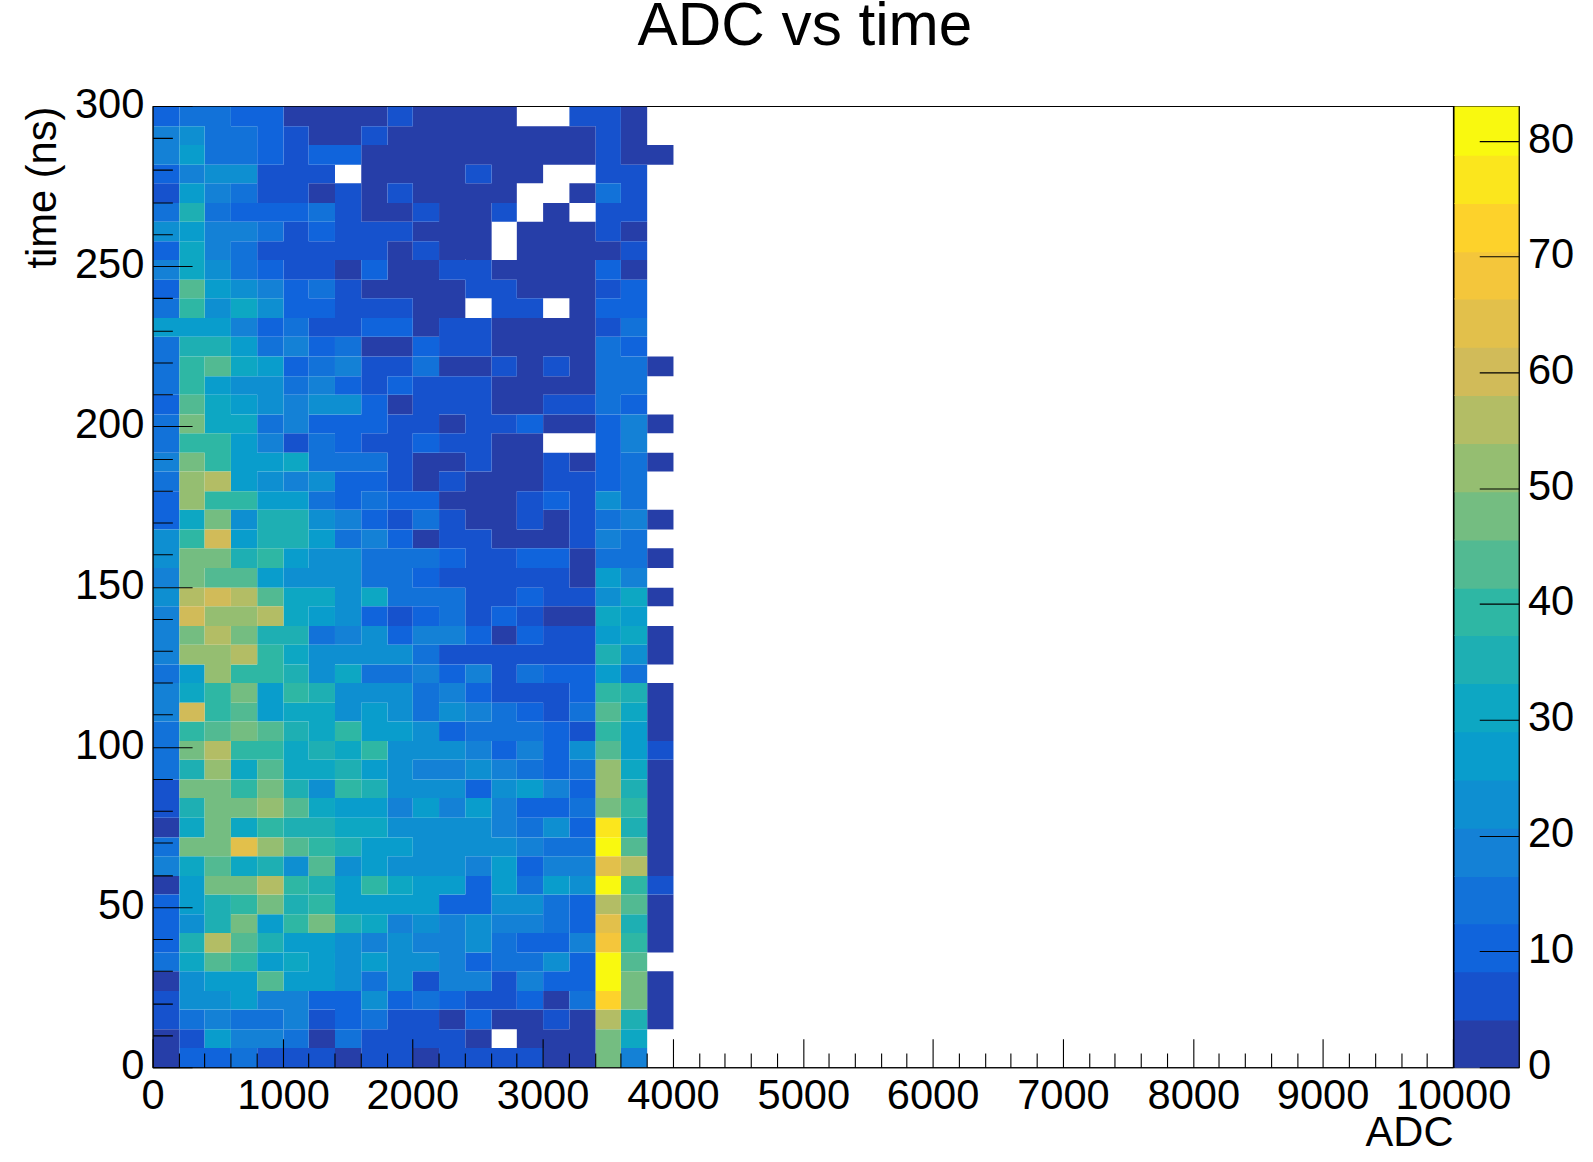
\includegraphics[width=0.45\linewidth]{figures/adc_versus_time_before_correction.png} &
            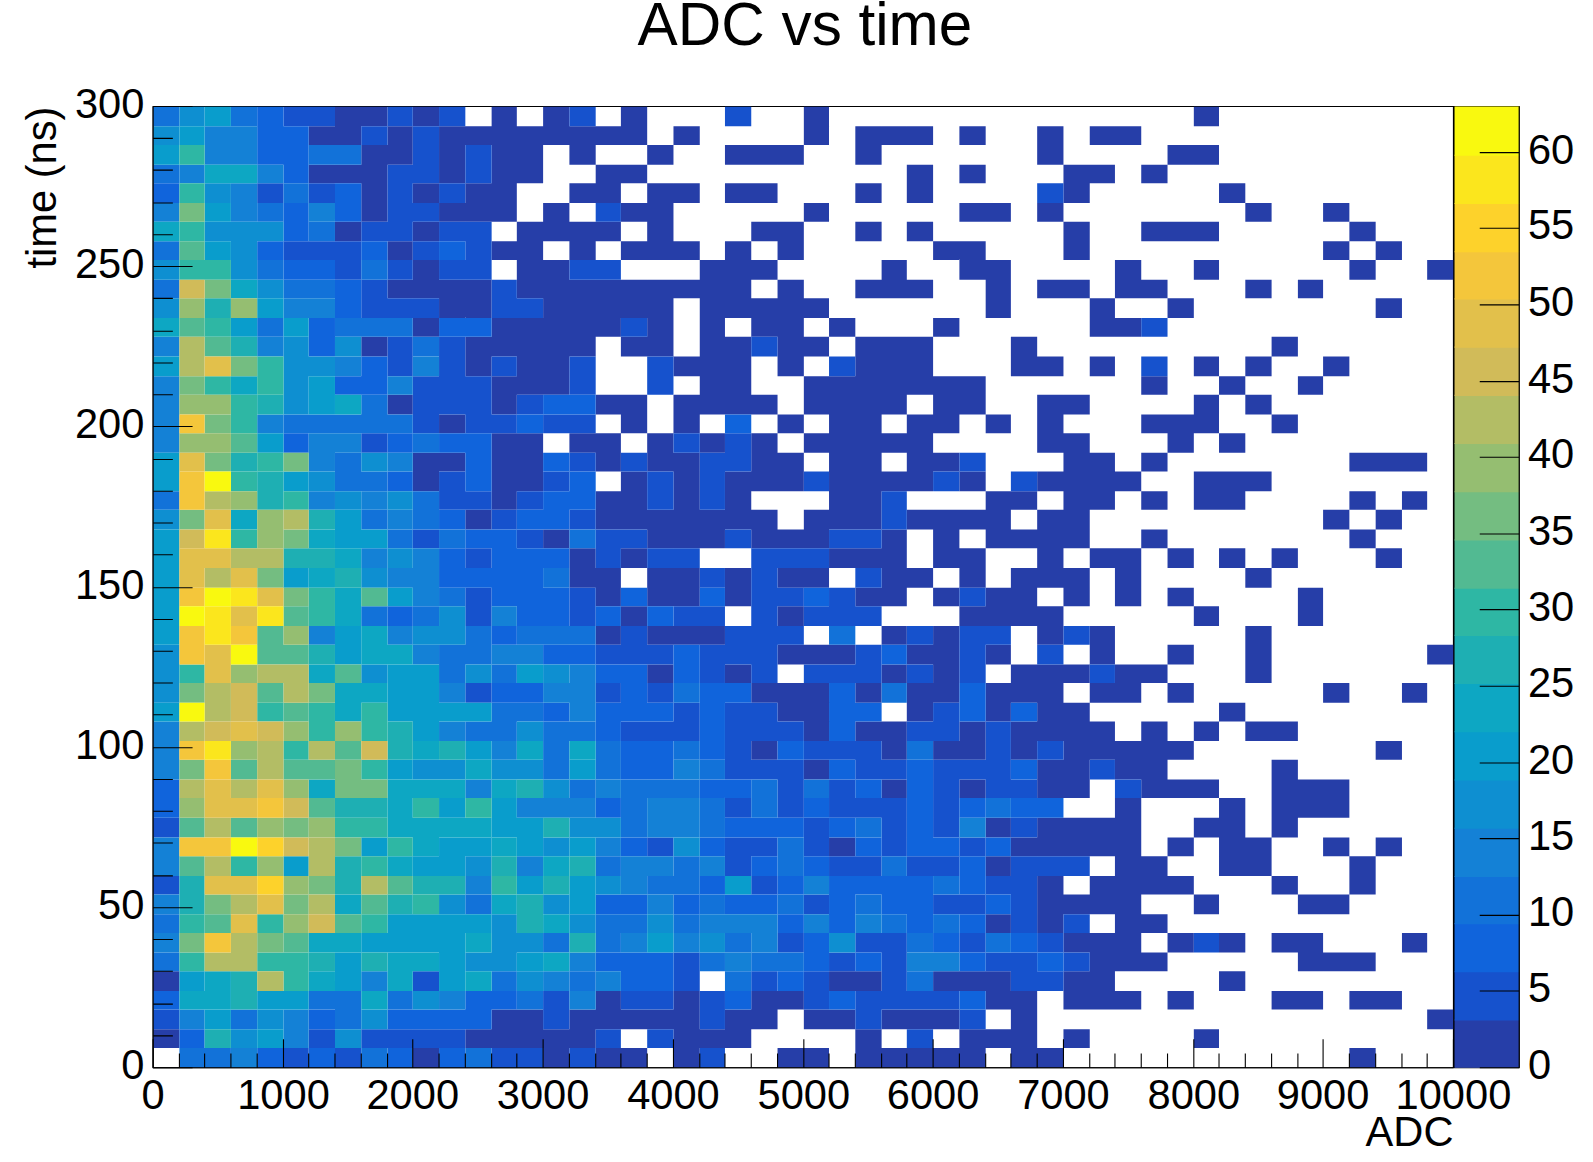
\includegraphics[width=0.45\linewidth]{figures/adc_versus_time_after_correction.png}
    \end{tabular}

\end{frame}

\begin{frame}{Results 2/2}
    \begin{itemize}
        \item We have earned some tracks.
        \item Stats for run 21476, 4He, 10.6 GeV
        \item Cuts: 1 electron, 1 track with nhits $>=7$ and chi2 $< 8$
    \end{itemize}

    \centering
    \vspace{0.2cm}

    {
        \renewcommand{\arraystretch}{1.5}
        \begin{tabular}{|c|c|c|}
            \hline
                    & coatjava dev & after adc correction \\
            \hline
            nb. tracks & 2244         & 2436 \\
            \hline
        \end{tabular}
    }

    \centering
    \vspace{0.5cm}

    \begin{tabular}{cc}
        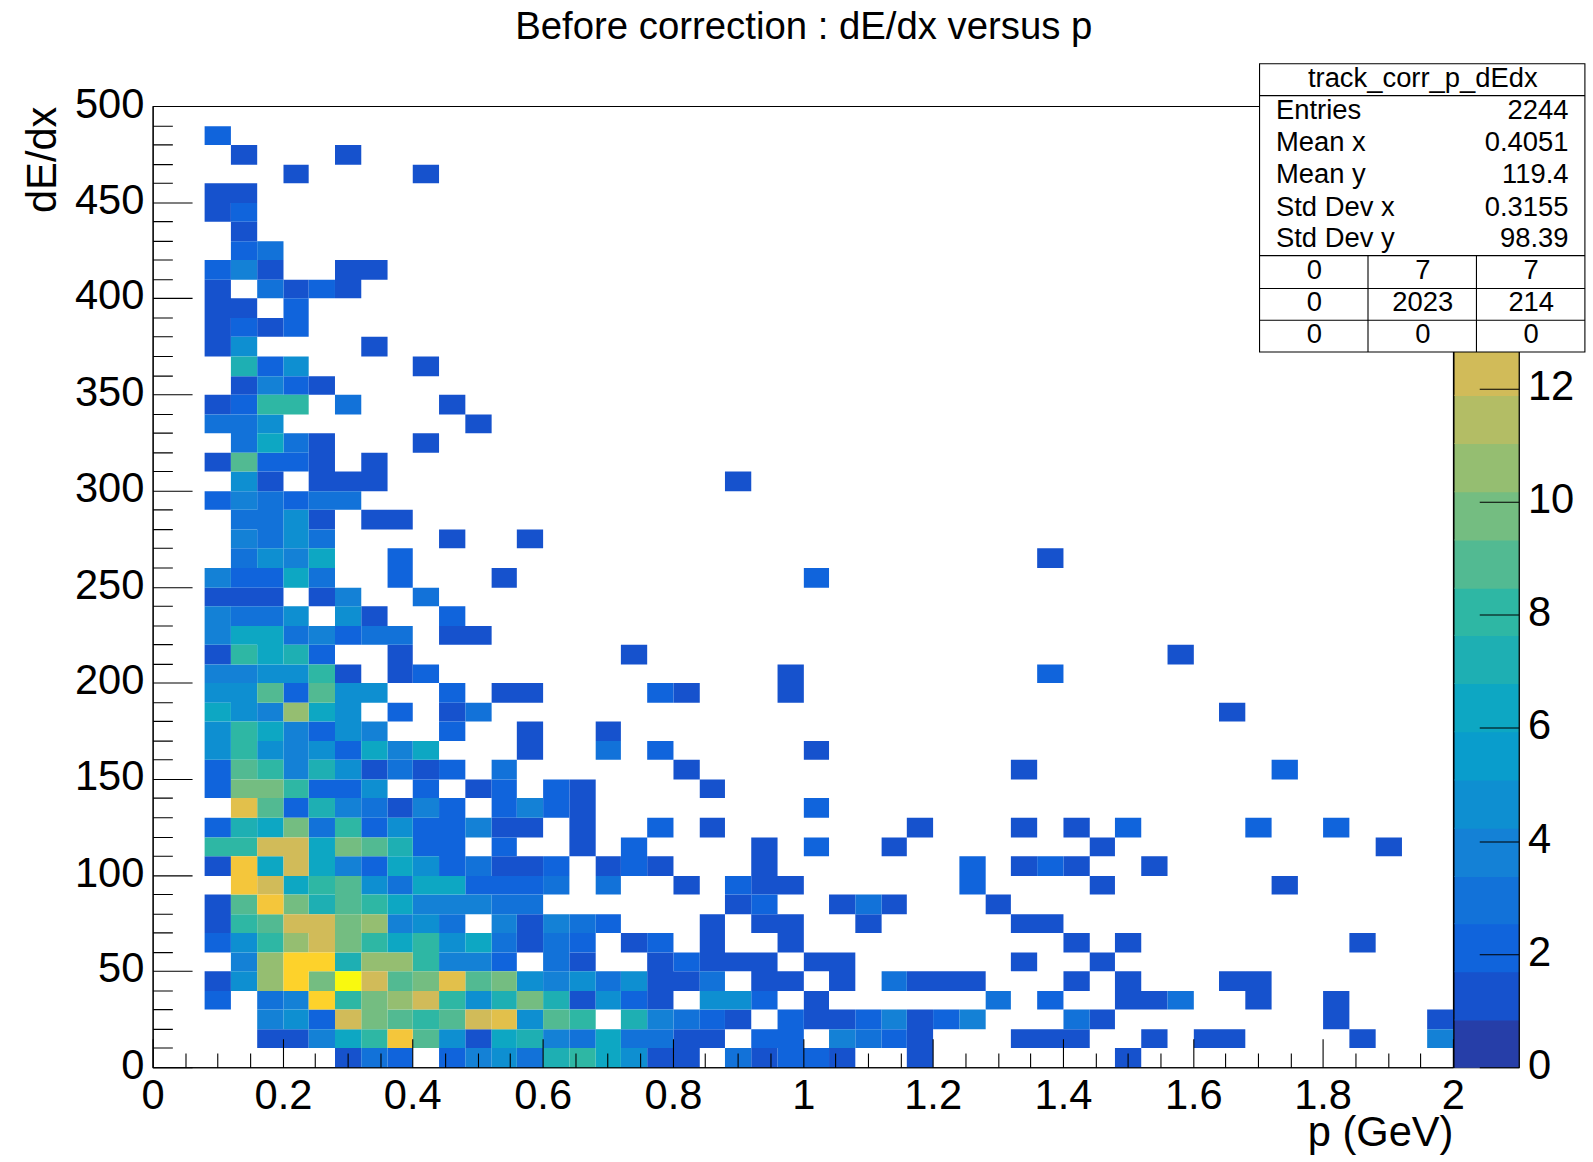
\includegraphics[width=0.45\linewidth]{figures/dEdx_before_correction.png} &
            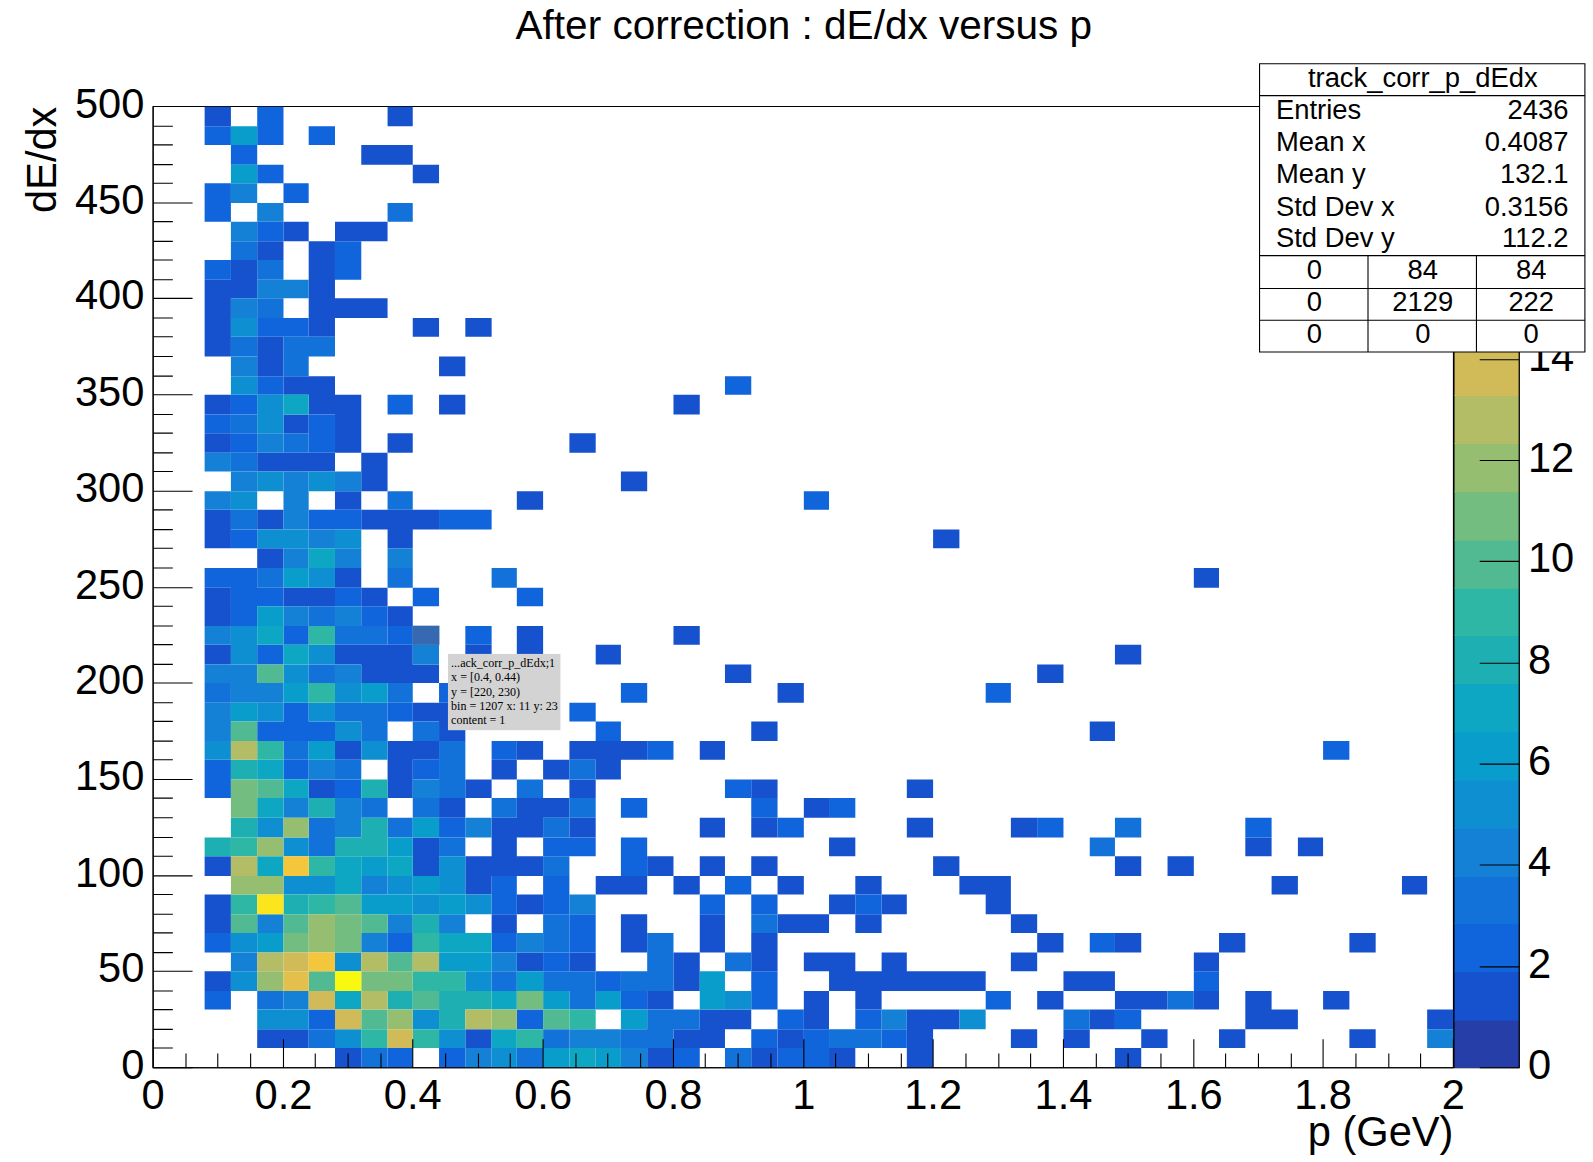
\includegraphics[width=0.45\linewidth]{figures/dEdx_after_correction.png}
    \end{tabular}

\end{frame}

\begin{frame}{Other approach}
    \begin{itemize}
        \item I selected good signals with $1800 < ADC < 3500$
        \item I compute the ToT at a fixed threshold : 2000
        \item For the same samples, I plot ADC versus ToT and versus Slope
        \item The ToT seems more precise than the Slope, but it is not linear!
        \item How should we extrapolate the ADC versus ToT relation ?
        \item I plan to study the ADC resolution for each method.
    \end{itemize}

    \centering
    \vspace{0.5cm}

    \begin{tabular}{cc}
        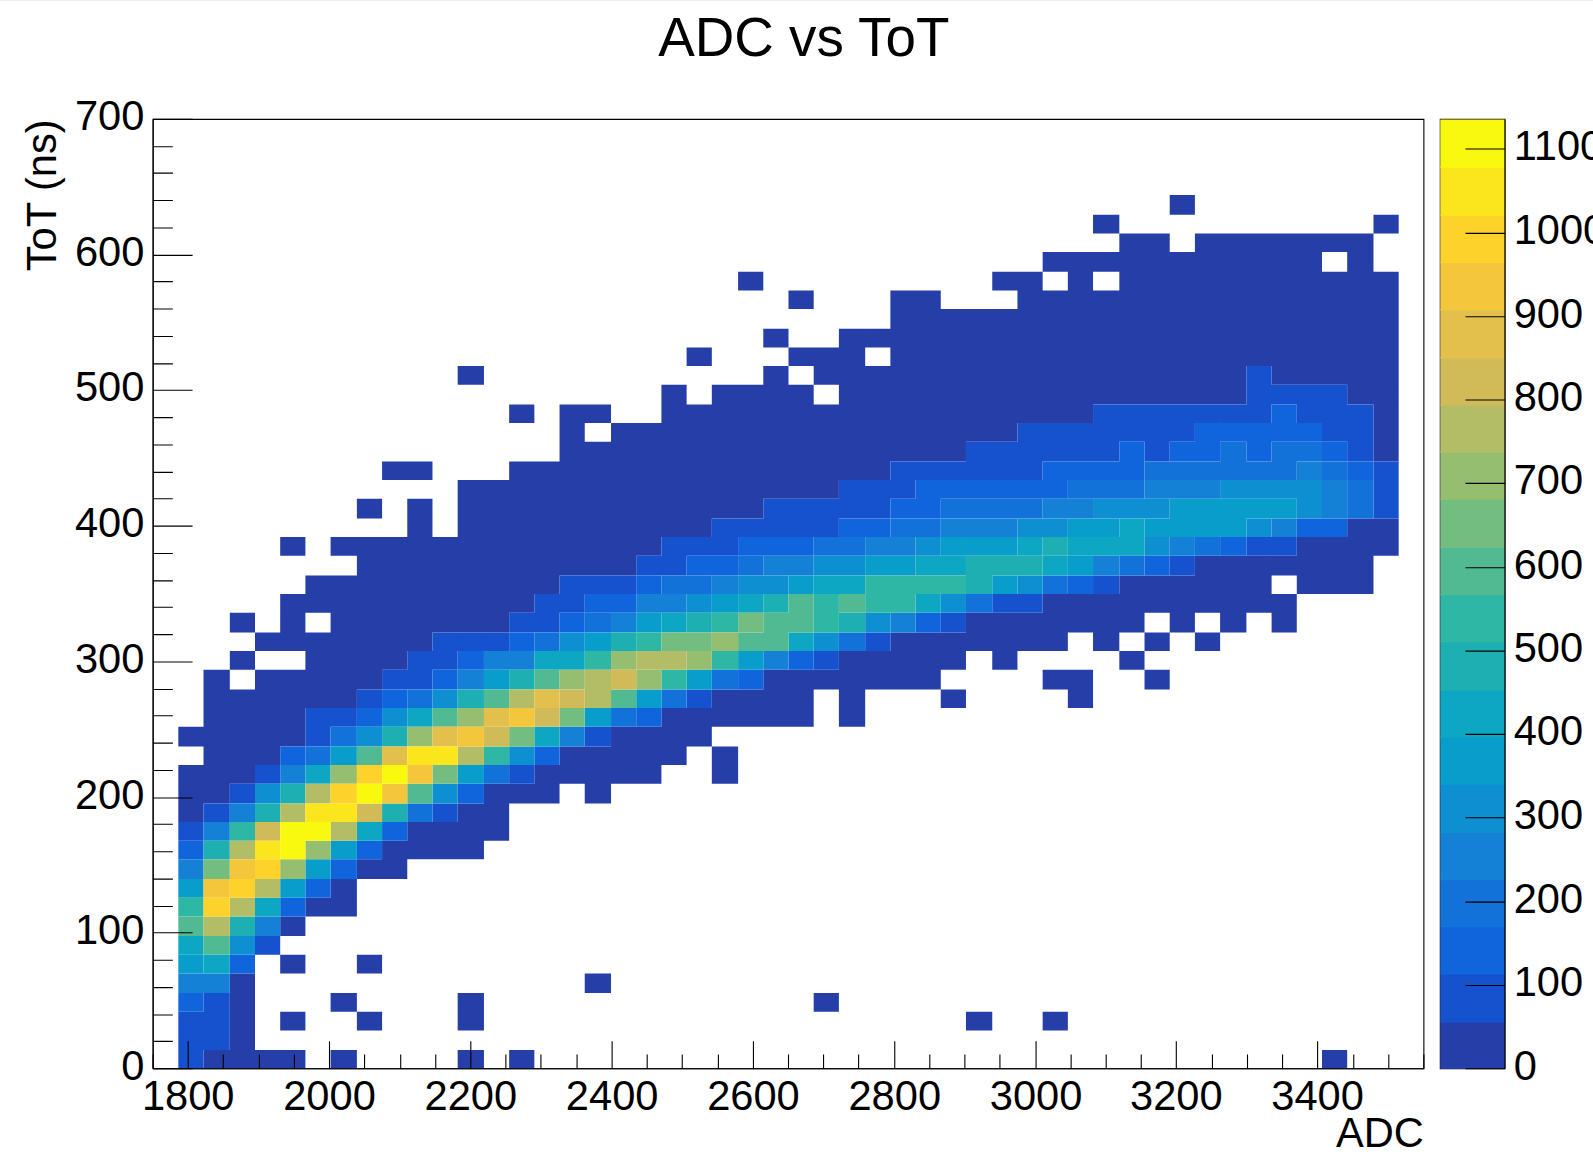
\includegraphics[width=0.45\linewidth]{figures/adc_versus_new_tot_specific_adc.png} &
            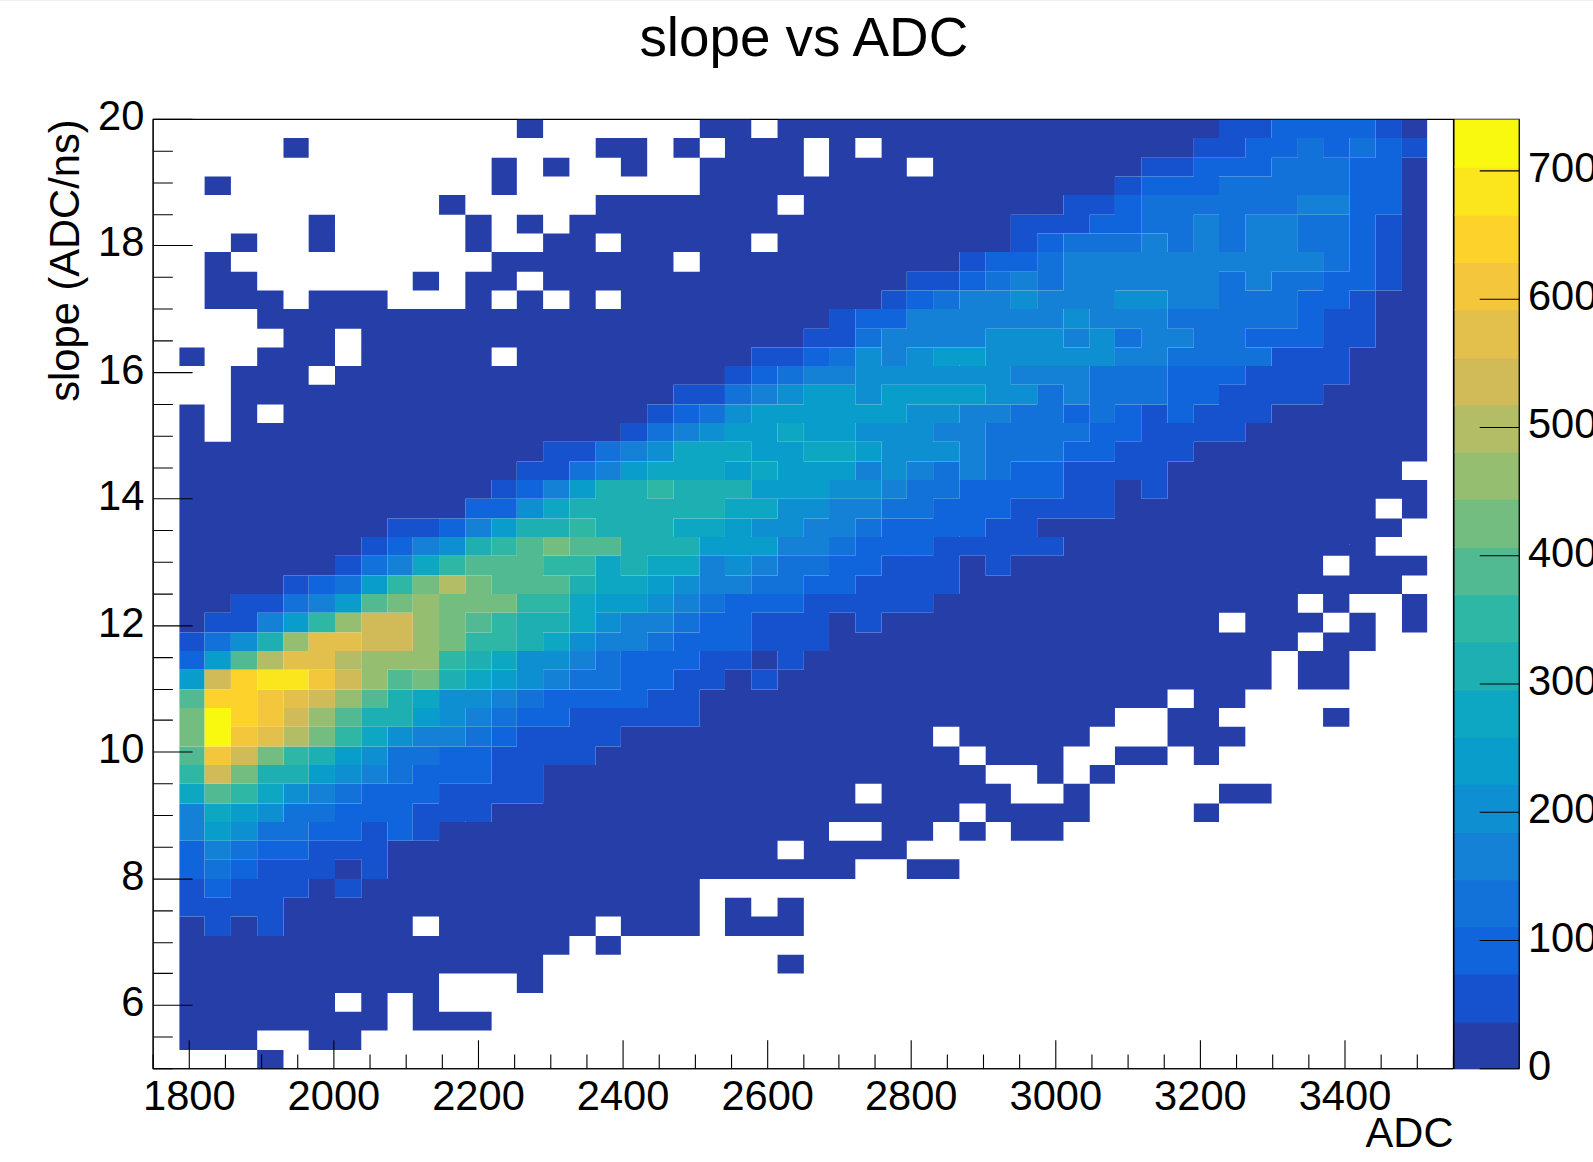
\includegraphics[width=0.45\linewidth]{figures/adc_versus_slope_specific_adc.png}
    \end{tabular}


\end{frame}


\begin{frame}{Backup slides}
    \begin{itemize}
        \item Bias in the time reconstruction of saturated signals
        \item For such signals, the arrival time and the timeOverThreshold can be wrong
    \end{itemize}

    \centering
    \vspace{0.2cm}

    \begin{figure}
        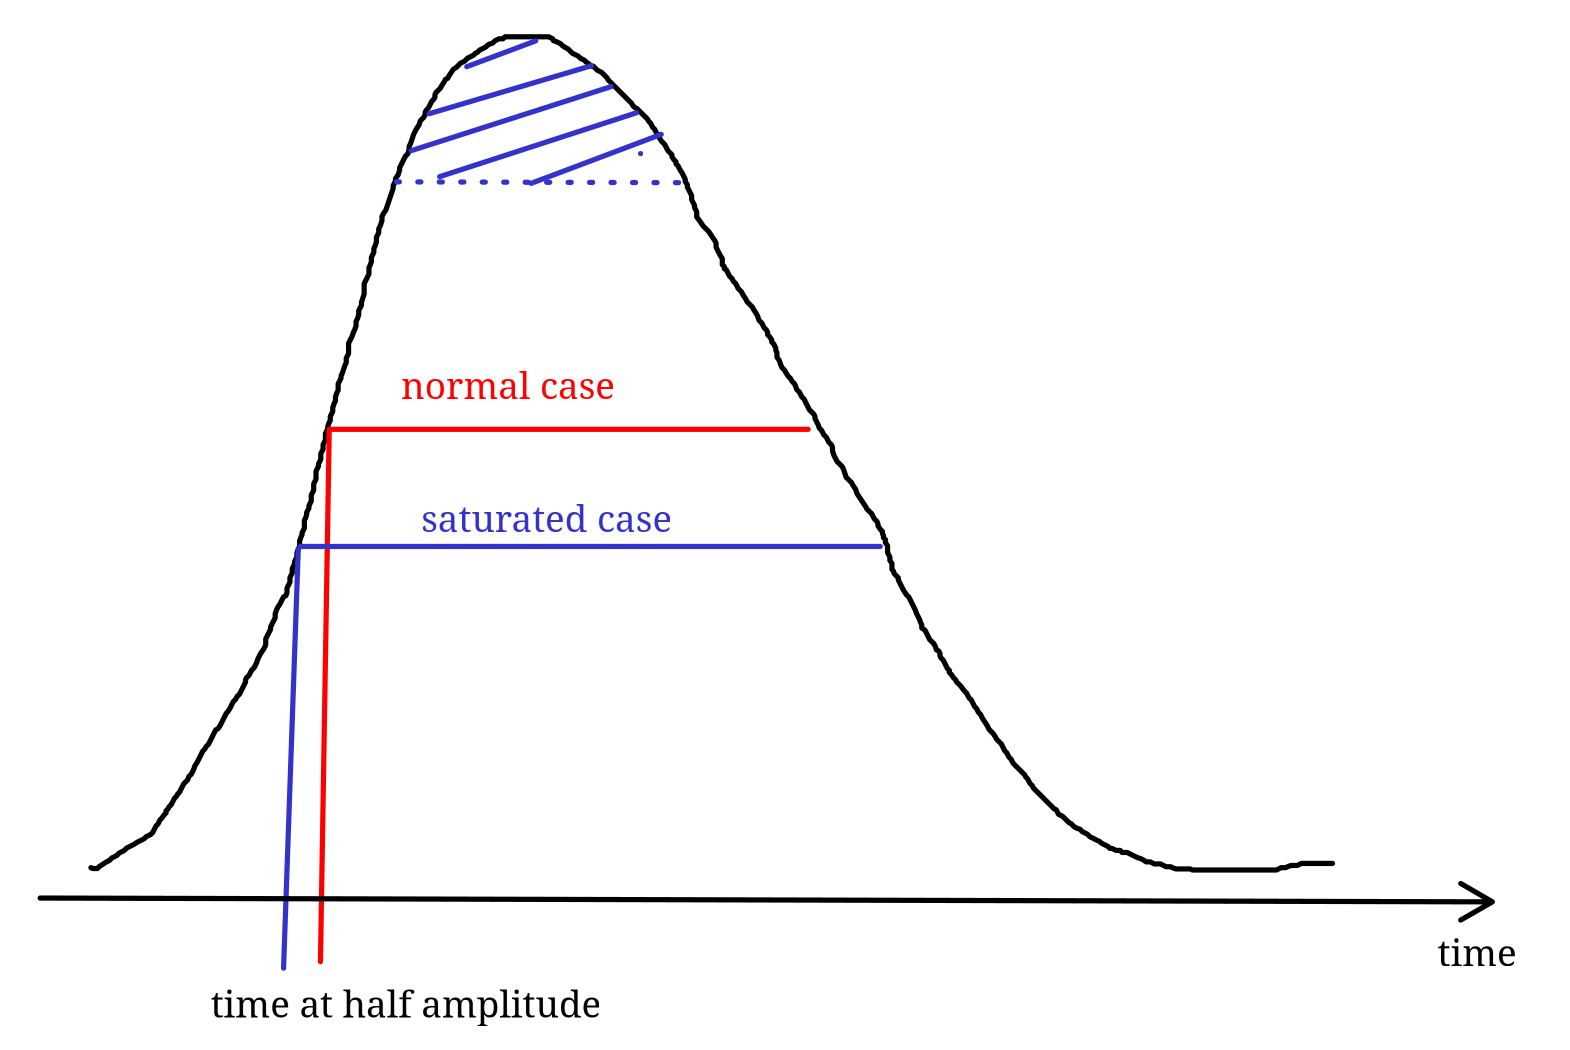
\includegraphics[width=0.65\linewidth]{figures/timewalk.png}
    \end{figure}

\end{frame}












\end{document}


